\section{Auswertung}
\label{sec:Auswertung}

\subsection{Threshold current measurement}

The procedure is the same as in chapter \ref{sec:alignmentSpeckle}. Both just below the threshold current and at it, a picture of the detector card is taken in each case. 
These can be found in figures \ref{fig:led} and \ref{fig:laser}. The threshold current is measured as $I_{thr} = 31.4 \,\si{\milli\ampere}$.

\subsection{Rubidium fluorescence and the transmission spectrum}

The procedure for this is also as described in \label{sec:DurchRubiFluor}. The current used here is $72.2 \,\si{\milli\ampere}$ and the piezo crystal is also switched on. 
The rubidium fluorescence can be seen in Figure \ref{fig:lumin}, the transmission spectrum on the function generator in Figure \ref{fig:peaks}.
Clearly seen here are the four expected peaks due to the absorption of rubidium. In the experiment itself, fine adjustments are made to ensure that there is no mode jump within this range that would falsify the result.
With reference to Figure \ref{fig:rubiAbs}, the peaks can be assigned from left to right to the transitions 87a, 85a, 85b, 87b.

\begin{figure}[H]
  \centering
  \includegraphics[width=.8\textwidth]{content/led_card.jpeg}
  \caption{The light image just before laser granulation occurs.}
  \label{fig:led}
\end{figure}

\begin{figure}[H]
  \centering
  \includegraphics[width=.8\textwidth]{content/laser_card.jpeg}
  \caption{The laser granulation at the setting of the threshold current}
  \label{fig:laser}
\end{figure}
\begin{figure}[H]
  \centering
  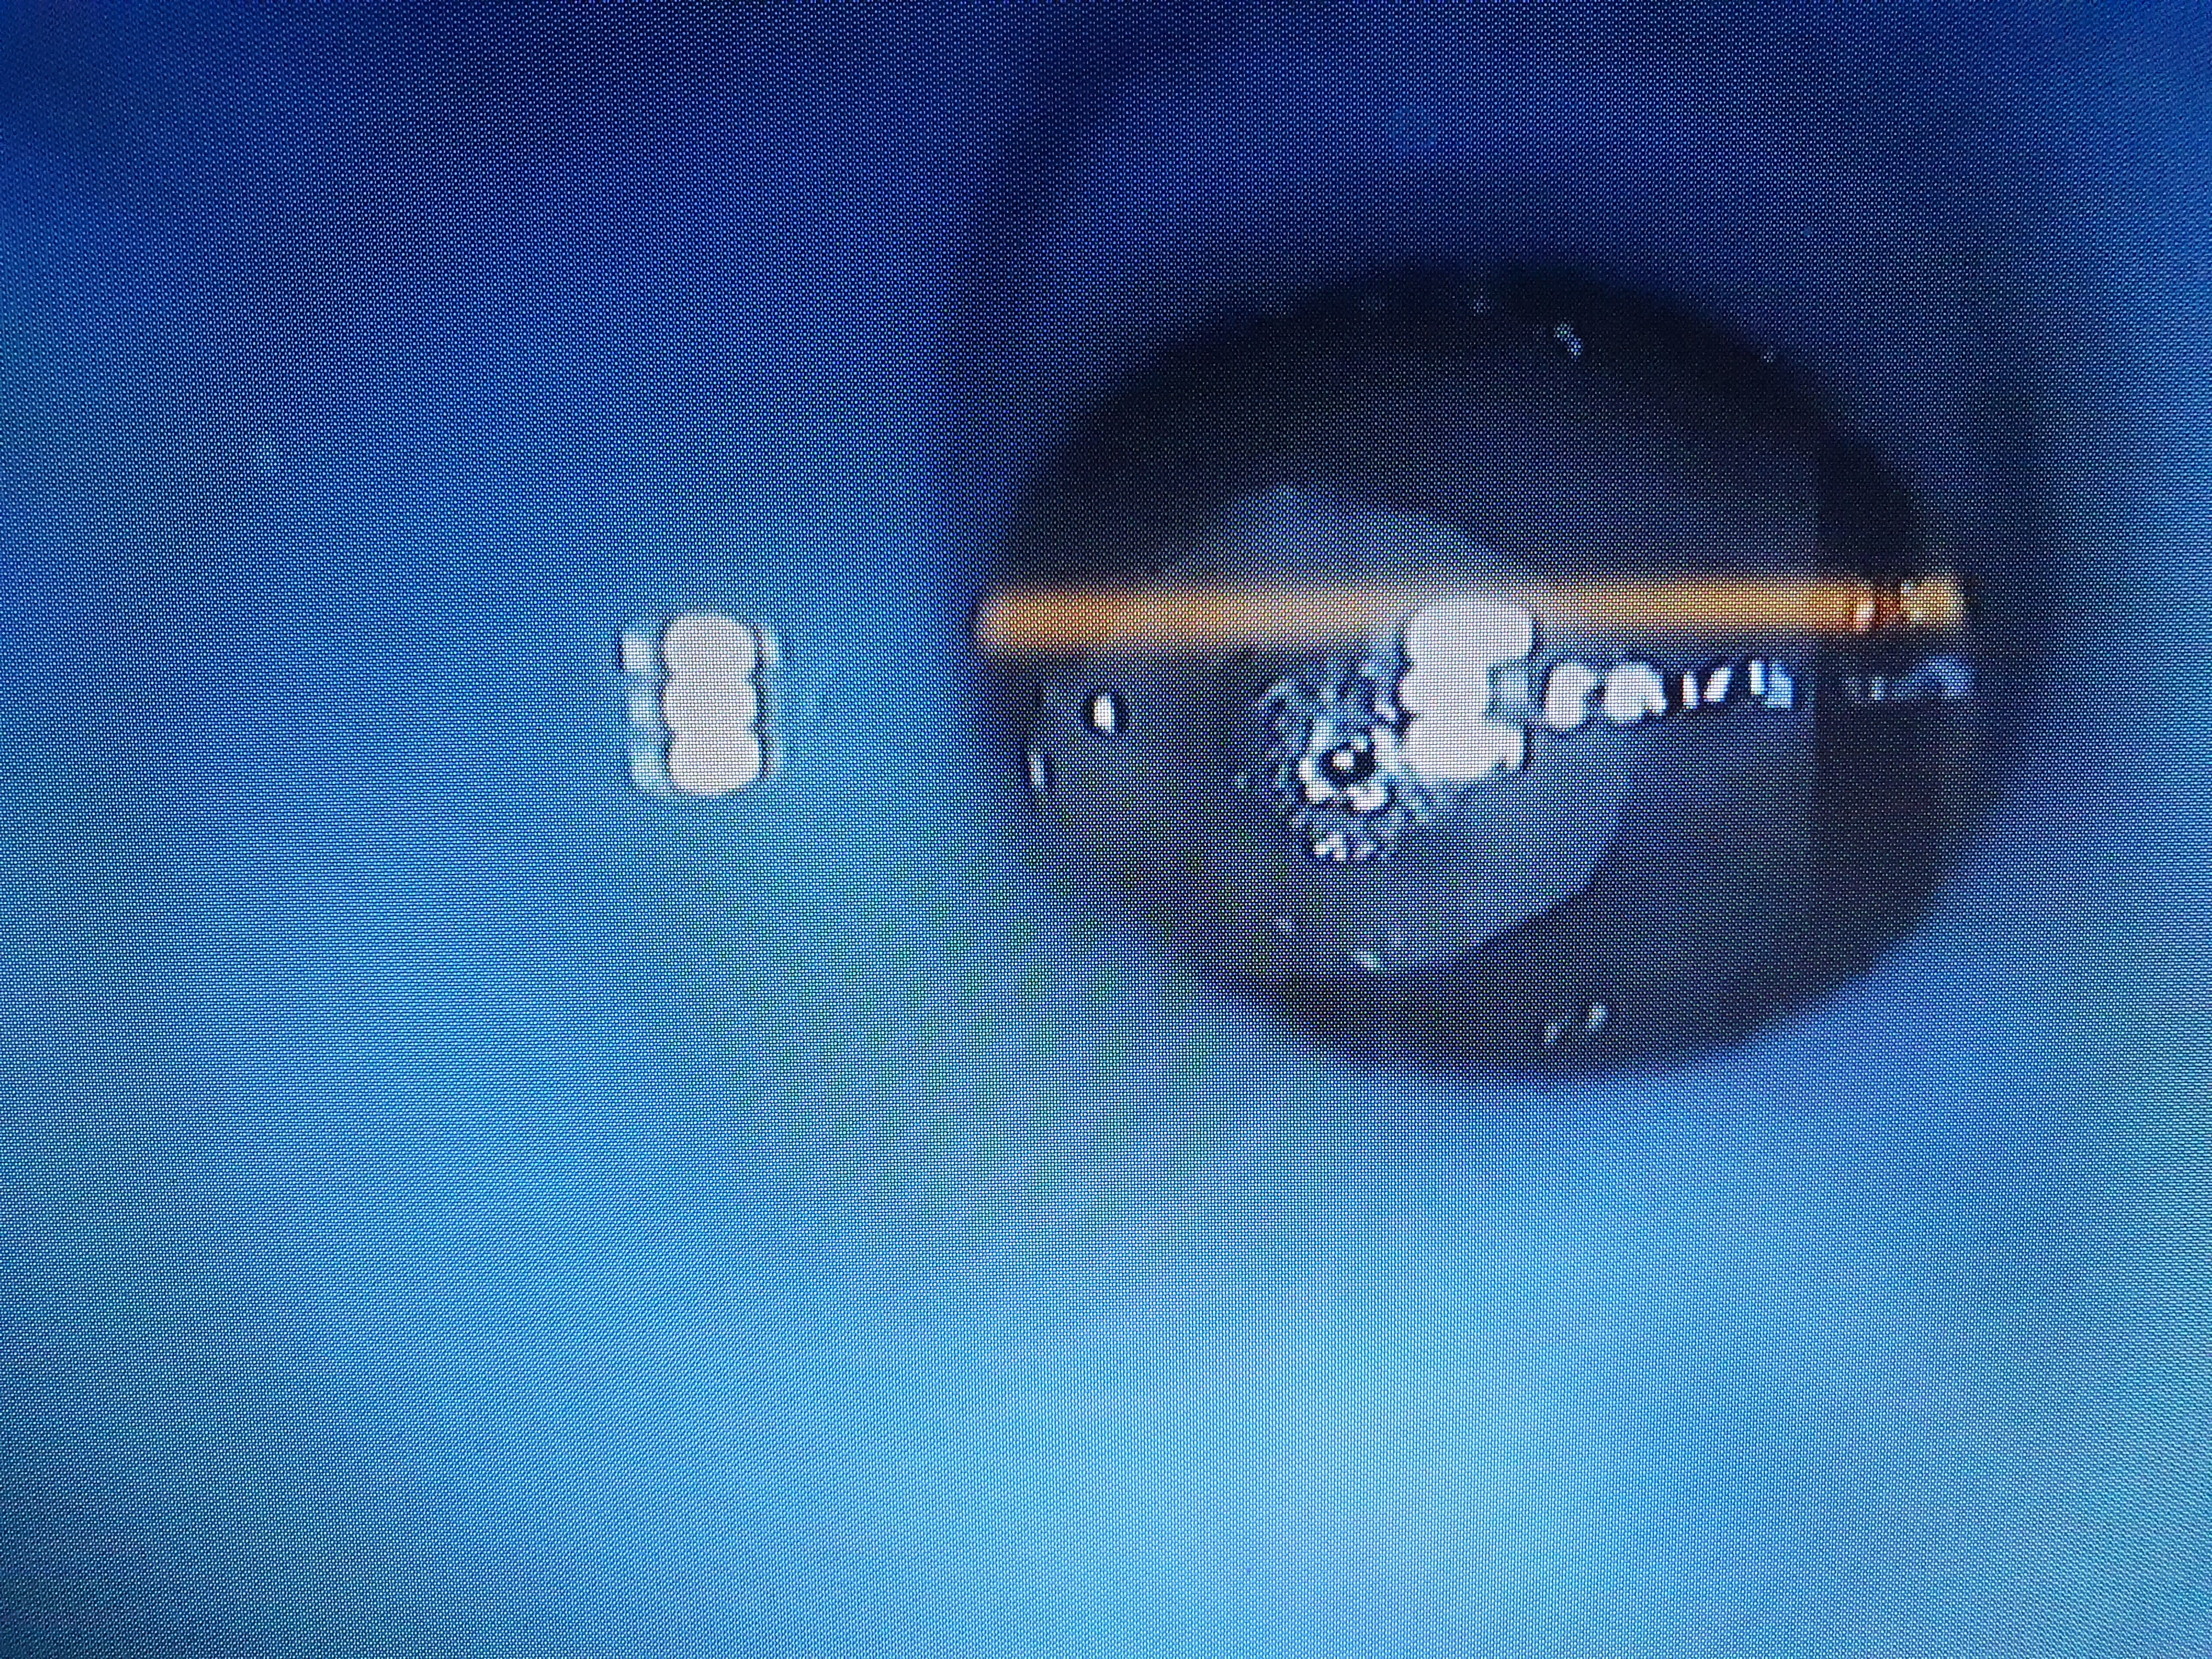
\includegraphics[width=.9\textwidth]{content/lumin.jpg}
  \caption{The observed rubidium fluorescence.}
  \label{fig:lumin}
\end{figure}
\begin{figure}[H]
  \centering
  \includegraphics[width=.9\textwidth]{content/peaks.jpg}
  \caption{The transmission spectrum with suppressed background.}
  \label{fig:peaks}
\end{figure}

